\subsection{The Compressed Size in One Table}
\label{sec:headline}

The rest of this section builds the comparison one factor at a time; its
outcome is in Table~\ref{tab:synthesis} and Fig.~\ref{fig:headline}. Both
start from one quantity: the compressed size of the HEALPix tile divided by
the compressed size of the area-matched \term{native UTM square}, at the same
reconstruction error, with no storage overhead charged to either side. A
value of $2$ means the HEALPix representation takes twice the bytes; $1$
means the two are the same size. The five \term{targets} run from a quarter of a
percent to a quarter of a typical scene's contrast, the median standard
deviation of the 40 tiles, $0.04$ in reflectance. The table gives five
things per \term{target}. The first is that ratio for the Clough--Tocher
\term{carrier} the paper uses; it is the column $\gamma_\star$, since the two
coincide (Section~\ref{sec:rd_main}). The second is the share of the raw
penalty that compression recovers. The third is the same \term{carrier} against
a native raster subjected to the half-pixel Clough--Tocher fixed-phase
smoothing control of Section~\ref{sec:support_controls}. The fourth is
the verdict over a range of native-layout overheads. The fifth is the
verdict at the illustrative $30\%$ overhead with its corrected
$p$-value. $n$ is the number of regions whose sweeps bracket the \term{target}
on both grids. The verdict column is within-representation: each grid is
scored against its own uncompressed raster. The HPX/sm.\ column is the
same comparison under a sensitivity control that reduces the
transfer-induced smoothing asymmetry, at one fixed phase rather than in
a phase-matched experiment. It stays above one at every \term{target}, so in
these controls geometry alone does not cross parity.
Section~\ref{sec:common_reference} charges the \term{transfer} and the \term{read} to
the \term{carrier} instead, and reaches the same place. The figure adds the
same tile rebuilt with the PSF-aware and inverse-distance \term{transfers} of
Section~\ref{sec:transfer_cost}, on the regions all three sweeps
bracket. Under an operational overhead $\gamma$ on the native product
every ratio at $\gamma=1$ divides by $\gamma$.

\begin{table*}[t]
\centering
\caption{The verdict per RMSE target: overhead-free ratio, critical overhead and the illustrative operating point}
\label{tab:synthesis}
\footnotesize
\setlength{\tabcolsep}{3pt}
\begin{tabular}{@{}lrrlrrrrrlrrl@{}}
\toprule
 & & \multicolumn{4}{c}{$\gamma=1$} & \multicolumn{3}{c}{HPX smaller (\% of $n$)} & & \multicolumn{3}{c}{$\gamma_{\mathrm{tile}}=1.3$} \\
\cmidrule(lr){3-6}\cmidrule(lr){7-9}\cmidrule(lr){11-13}
Target RMSE & $n$ & $\gamma_\star$ & IQR & $f(e)$ &  HPX/sm. & $\gamma{=}1$ & $\gamma{=}1.3$ & $\gamma{=}2$ & Inconclusive $\gamma$ & Ratio & $p_{\mathrm{Holm}}$ & Verdict$^{*}$ \\
\midrule
$10^{-4}$ & 40 & 2.07 & [1.99, 2.16] & 0.32 & 2.22 & 2 & 2 & 28 & $2.03$--$2.10$ & 1.59 & $<10^{-4}$ & UTM \\
$3\times10^{-4}$ & 40 & 1.95 & [1.74, 2.05] & 0.40 & 2.10 & 5 & 8 & 70 & $1.76$--$1.97$ & 1.50 & $<10^{-4}$ & UTM \\
$10^{-3}$ & 39 & 1.58 & [1.22, 1.90] & 0.64 & 1.83 & 13 & 28 & 92 & $1.35$--$1.72$ & 1.21 & 0.016 & UTM \\
$3\times10^{-3}$ & 37 & 1.23 & [0.97, 1.56] & 0.86 & 1.48 & 27 & 59 & 97 & $1.08$--$1.34$ & 0.94 & 0.187 & inconcl. \\
$10^{-2}$ & 32 & 0.93 & [0.89, 1.03] & 1.04 & 1.24 & 69 & 94 & 100 & $0.90$--$0.99$ & 0.72 & $<10^{-4}$ & HPX \\
\bottomrule
\end{tabular}

\end{table*}


\begin{figure}[t]
\centering
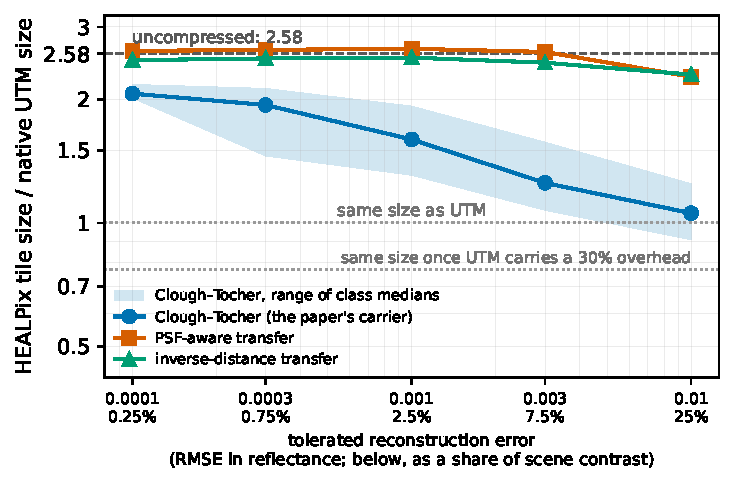
\includegraphics[width=\columnwidth]{figures/fig_headline}
\caption{Compressed size of the HEALPix tile relative to the native UTM
square, at equal reconstruction error and with no overhead on either side,
for the three transfers used to fill the tile. The shaded band is the
range of the four land-cover class medians for the Clough--Tocher
carrier; the curves have the populations of Table~\ref{tab:synthesis}
and Section~\ref{sec:transfer_cost}. The dashed line is the uncompressed ratio; the
dotted lines mark parity with no overhead and with the illustrative $30\%$
overhead on the native product.}
\label{fig:headline}
\end{figure}

Three things follow. First, the tolerated error sets the ratio.
Uncompressed, the tile is $2.58$ times the square. Compressed, the ratio
is $2.06$ when the reconstruction must stay within $10^{-4}$ of the stored
values, a quarter of a percent of a typical scene's contrast. It falls
steadily to $0.93$ at $10^{-2}$, a quarter of the contrast, where the
HEALPix tile is the smaller one before any overhead is charged. The
oversampling penalty is then more than recovered by the codec, though
only at an error that is large for a reflectance product. Second, the
kind of scene moves the ratio less than the tolerated error does. Across
the four classes the medians span $2.01$--$2.17$ at the tightest \term{target}
and $0.89$--$1.10$ at the loosest, and no class changes the picture.
Third, the way the tile was filled matters as much as everything else
combined, and the three \term{transfers} are not interchangeable. The
Clough--Tocher \term{transfer} adds no information that was not in the native
pixels; it does smooth them. The PSF-aware \term{transfer} of the companion
study~\cite{delouis2026resample} is designed to undo part of the
instrument blur and estimate a sharper latent field, whose
reconstruction gain that study establishes under its own conditions. A
codec asked to preserve the content it places on the tile must spend
bytes on it. The tile compresses to $2.3$--$2.6$ times the \term{UTM square} at
every \term{target}, close to the uncompressed ratio, and the gap remains large
over the range of native-layout overheads examined here, the
illustrative $\gamma_{\mathrm{tile}}=1.30$ included. Those bytes buy
content the Clough--Tocher tile does not hold, so the two ratios answer
different questions (Section~\ref{sec:transfer_cost}). The
inverse-distance average, which restores no detail at all, costs nearly
as much ($2.1$--$2.5$), so the extra bytes are consistent with the price
of leaving the smooth interpolant. With a Clough--Tocher \term{carrier}, the
storage question is therefore a question of the tolerated error.
Sections~\ref{sec:rd_main}--\ref{sec:rd_illustrative} show where the
answer changes sign: at $10^{-2}$ at equal layout overhead, more exactly
for any relative overhead $\gamma\ge0.93$, and one \term{target} earlier once
a $30\%$ overhead is charged to the native product. A reader whose
product carries an illustrative $30\%$ layout overhead reads the
Clough--Tocher ratio as $1.59$ down to $0.72$ (last block of
Table~\ref{tab:synthesis}), and the PSF-aware one as $1.8$ to $2.0$.
